A semantic role labeling (SRL) system for Chinese was reported by \cite{you-chen:2004}. Input to the system was a parse tree, parsed by Sinica Chinese parser\footnote{An online demo of the parser is available at http://parser.iis.sinica.edu.tw/}, and output was its semantically labeled counterpart. Sinica Treebank \cite{sinica-treebank}, a semantically annotated Chinese treebank, was used to train simple probabilistic models, which were used for semantic role classification. As far feature set, the system relied on a number of conventional lexical (e.g. \verb+head_word+, \verb+head_word_pos+, \verb+target_word+, \verb+target_word_pos+) as well as syntactic features (e.g. \verb+phrase_type+, \verb+position+). The overall accuracy of the system was reported to be 92.71\%. Even though this accuracy can be considered on the higher side, there was room for improvement, especially in two subtasks: data sparseness handling and classification approach. \\
Data sparseness handling first, the old system used a back-off strategy to tackle this problem (see \cite{you-chen:2004} for more details). This considerably improved the baseline performance, but data sparseness still remained an issue. A major reason was dependency of the system on non-generalized lexical features (e.g. \verb+head_word+, \verb+target_word+). 
%As \cite{Gildea:2002} pointed out that lexical features, though very useful for semantic role labeling, may pose the issue of data sparseness. To handle this, they proposed a number of methods to generalize the lexical statistics including the use of a semantic hierarchy -- WordNet. However, they restricted their approach to the generalization of the head words of noun phrases only. Later, \cite{Lin:2010:CSR:1909632.1912231} experimented by extending it other lexical features, such as first word, last word etc, and witnessed improvements. 
In this paper, we used E-HowNet \cite{keylist}, a semantic knowledge-base for Chinese, to generalize two lexical features (i.e. \verb+head_word+ and \verb+target_word+), and hence, to better address the data sparseness concern.\\ 
Classification methodology next. In the old system, simple probabilistic models, together with a back-off strategy, were used for semantic role assignment. As shown below, a particular feature combination was used for each model, and the backing-off was based on number of examples seen in the training data.
\begin{verbatim}
if#of(h,h_pos,t,t_pos,pt,position)
                       >threshold
 P(r|constituent)=
 P(r|h,h_pos,t,t_pos,pt,position)
else
 if#of(h_pos,t,t_pos,pt,position)
                      >threshold
  P(r|constituent)=
  P(r|h_pos,t,t_pos,pt,position)
else
......
%\end{verbatim}
%A critical observation is that backing-off based on a constant threshold value did not allow to exploit the statistical knowledge in the best possible way. The reason is that if enough examples, with a more constrained feature combination, have been seen in the training data, it did not allow to utilize the less constrained statistical information, which may suggest a more probable role (see Section 4.3 for an example). We propose a different strategy that is based on a combination of weighted simple probabilistic models. In our method, both more and less constrained probabilities are ranked by learned weights, and then the top ranked information is used for final decision making. The probabilities are calculated using the same training data (i.e. Sinica treebank), and optimal weights, which encode the worth of a particular feature combination in determining the semantic role, are found using genetic algorithms. To show the effectiveness of our idea, we build a number of systems that are based on other well established classification approaches (e.g. NaiveBayes, Decision Trees, Maximum Entropy, Linear Interpolation), and compare their outcomes to our system. The experimental results show that our strategy outperformed all other systems including the previous system, and lead to a considerable improvement in the accuracy of our final SRL system.\\
%To further enhance the performance, we also add a number of features to the feature set of the system, and propose a number of heuristic rules (see Section 2 and 5 respectively for further details).\\
%The rest of the paper is organized as follows: Section 2 briefly outlines our feature set, and reports how we have generalized the lexical features. This is followed by a description of probabilistic models in Section 3. Section 4 explains our classification method with the help of an example. Experiments and evaluation results are given in Section 5, which is followed by conclusion and future work section.     
\section{Feature Set}
In addition to the set of lexical and syntactic features, mentioned in the introduction section and used by \cite{you-chen:2004}, we have used the following features:
\begin{itemize}

\item \verb+pos_left_right_child:+ part of speech tags of the immediate left and right siblings of a test node.
\item \verb+passive:+ A sentence-level boolean feature indicating weather the sentence, containing the test node, is passive or not.
\item \verb+all_pos:+ A set of part of speech tags of all nodes under a test node including the test node itself.
\item \verb+all_semType:+ A set of semantic types of all nodes of the tree, the test node is a child of.
\end{itemize}
As pointed out by \cite{Gildea:2002}, lexical statistics, though very useful for semantic role labeling, often becomes a source of data sparseness. This is because, for a particular test case, the lexical values may not have been seen in the training data due to a large vocabulary size. 
%As an example, take two test cases with the feature set ($h\_word$, $h\_word\_pos$, $t\_word$, $t\_word\_pos$, $pt$, $position$) and with the following corresponding values:
%\begin{verbatim}
%(a) ...,N,...,N,NP,1
%(b) ...,N,...,N,NP,1
%\end{verbatim}
%Considering that, the particular head and target words in (a) have been, and in (b) have not been seen in the training data, the system will assign a semantic role to candidate (a), while failing to assign a role to candidate (b) unless we use some back-off or any other data sparseness handling strategy. One such strategy is generalization of the lexical features. 
In our system, we have generalized two lexical features (i.e. \verb+head_word+, and \verb+target_word+) by replacing them with more general features (i.e. \verb+semanticType_head_word+ and \verb+semanticType_target_word+ respectively) extracted from the Chinese semantic knowledge-base (E-HowNet). \\
E-HowNet is an entity-relation model in which words have been grouped together based on their semantic relationships. This grouping, in other words, provides a way to generalize the lexical features, and hence can be used to solve the data sparseness issue.\\
%Now, if we use E-HowNet, the head words in (a) and (b) will generalize to one semantic type ?, and the target words to the semantic type ?. 
Table 1 gives coverage statistics of each model (see Section 3 for details about the models) before and after adding these generalizations. As can be seen, after generalization, the coverage improved considerably for each model, which ultimately resulted in better performance.
\begin{table}[!h]
\begin{center}
\begin{tabular}{|p{1cm}|c|c|}
\hline \bf Model & \bf Before & \bf After \\ \hline
 1 & 7.10\% & 12.68\%  \\ 
 2 & 52.06\% & 73.05\%   \\ 
 3 & 67.43\% &  82.68\%   \\ 
 4 & 74.56\% &  93.35\%  \\ 
 5 & 97.97\% & 97.97\%   \\ 
 6 & 28.60\% &  64.20\%   \\ 
 7 & 76.30\% & 94.23\%   \\ 
 8 & 82.97\% & 96.85\%   \\ 
 9 & 99.78\% & 99.78\%   \\ 
 10 & 90.09\% & 99.00\%   \\ 
\hline 
\end{tabular}  
\caption{Coverage Statistics}
\end{center}
\end{table}
\section{Probabilistic Models}
Ten simple probabilistic models, each based on a particular feature combination, were build using the Sinical treebank labeled data. The probabilities for each model were estimated using the following simple formula. 
\begin{Verbatim}[commandchars=\\\{\},codes={\catcode`$=3\catcode`_=8}]
  $P(r|constituent)$  
   $= P(r|f_{c})$
   $= #(r,f_{c})/#f_{c}$
\end{Verbatim} 
Where $f_c$ represents a particular feature combination. A number of combinations were tried, and for the final system we used the following set of ten combinations.
%\begin{verbatim}
\begin{verbatim}
{(semType_h_word,h_pos,
semType_t_word,t_pos,pt,position,
all_pos,passive,all_semType,
left_right_child_pos), 
(h_pos,semType_t_word,t_pos,pt,
position,passive),
(semType_h_word,h_pos,t_pos,pt,
position,passive),
(semType_t_word,t_pos,pt,passive,
position),
(h_pos,t_pos,pt,position,passive),
(semType_h_word,semType_t_word,
pt,position,passive),
(semType_t_word,t_pos,pt,passive),
(semType_t_word,t_pos,passive),
(t_pos,pt,position,passive),
(semType_t_word)}
\end{verbatim}
\section{Classification Method}
\subsection{Notations}
\begin{itemize}
\item Let $F$ be the set of feature combinations (given in the previous section), and $f_c$ be an element of $F$
\item $P$ be the set of corresponding probabilistic models, and ${P_f}_c$ be an element of $P$ with feature combination $f_c$ 
\item ${D_f}_c$ be the probability distribution computed by ${P_f}_c$ 
\item $M_{((p,r)|f_c)}$ be the most probable $(probability,role)$ pair from  ${D_f}_c$
\item $W$ be a set of optimal weights, $w$ be an element of $W$, and $wp$ be a weighted probability (i.e. rank)
\end{itemize} 
\subsection{Algorithm}
Our classification algorithm is as follows:
\begin{enumerate}
\item For a test candidate, extract values of all features (mentioned in section 2) using the parse tree and E-HowNet.
\item initialize $potential\_roles$  $\leftarrow$ $empty$ 
\item For each $f_c$  $\in$ $F$ do:
\begin{itemize}
 \item Find probability distribution ${D_f}_c$ using the corresponding ${P_f}_c$ model
 \item Select $M_{((p,r)|f_c)}$ from ${D_f}_c$
 \item Rank $M_{((p,r)|f_c)}$ by multiplying $p$ with the corresponding $w$ from $W$
 \item Append $(wp,r)$ to $potential\_roles$
 \end{itemize}
\item Return the top ranked $r$ from $potential\_roles$
 \end{enumerate}
%There are various well-established classification approaches that have been successfully used for the task of semantic role classification. \cite{Pradhan04shallowsemantic} used vector machines for this purpose, \cite{Zapirain:2007:USS:1621474.1621551,Lin:2010:CSR:1909632.1912231} used maximum entropy models, \cite{Gildea:2002} used simple probabilistic models together with different merging techniques, and \cite{you-chen:2004} used simple probabilistic models together with a back-off strategy for the same purpose. In this paper, we propose a slightly different classification approach, which is based on weighted simple probabilistic models. The major idea is as follows: \\
%For a test constituent, a list of most probable roles, each determined by one of the ten models (mentioned in the previous section), is build first. Then, these roles are ranked by multiplying them with weights, and finally, the top ranked role is assigned to the test constituent. The optimal weights, which encode the reliability factor, are found using genetic algorithms and a held-out development data set.\\
\subsection{An Example}
Suppose we want to assign a semantic role to the circled node of the parse tree given in Figure 1.
\begin{figure}[!h]
\centering
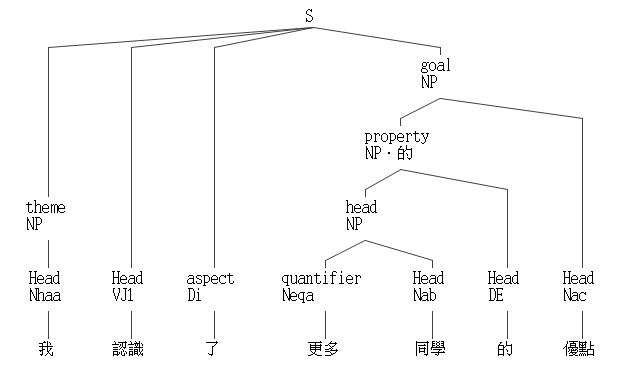
\includegraphics[width=.5\textwidth,height=3.5cm]{./examples/example3.png}
\caption{An example parsed sentence}
%\label{fig:example2-full}
\end{figure}
\noindent First, we have to extract the full set of \verb+(feature:value)+ pairs for the target test node. The extracted set is given below:
\begin{verbatim}
{(semType_h_word:advantage),
(h_pos:Nac),(semType_t_word:human),
(t_pos:NP??),(pt:NP),(position:-1),
(all_pos:NP??-NP-Neqa-Nab-DE),
(passive:False),
(left_right_child_pos:empty-Nac),
(all_semType:
BecomeMore-human-tool-advantage)}
\end{verbatim}
%semType\_h\_word:naming\\VG1,respective,NP,S,1,NP-VH11-VH11-VH11-DE-Nv1,True,VG1-empty,concession-name-tool-naming-black-white-3rdPerson-respective. 
The probability distribution estimated by each of the ten probabilistic models is given in Table\footnote{Note that due to sparseness of the training data, their is no probability distribution for the feature combination of model 1.} 2.

\begin{table}[!h]
\small
\begin{tabular}{|l|p{6.3cm}|}
\hline \bf ${P_f}_c$ & \bf  Probability Distribution (${D_f}_c$) \\ 
\hline 1 &  \\ 
\hline 2 & [(0.5072, 'possessor'), (0.4783, 'property'), 0.0145, 'quantifier')]\\ 
\hline 3 & [(0.5, 'property'), (0.5, 'possessor')] \\ 
\hline 4 & [(0.5035, 'property'), (0.4894, 'possessor'), (0.0071, 'quantifier')] \\ 
\hline 5 & [(0.8514, 'property'), (0.1361, 'possessor'), (0.0083, 'quantifier'), (0.0042, 'apposition')]\\ 
\hline 6 & [(0.5, 'property'), (0.5, 'possessor')]\\ 
\hline 7 & [(0.5035, 'property'), (0.4894, 'possessor'), (0.0071, 'quantifier')] \\ 
\hline 8 & [(0.5035, 'property'), (0.4894, 'possessor'), (0.0071, 'quantifier')]\\ 
\hline 9 &[(0.8598, 'property'), (0.1240, 'possessor'), (0.0132, 'quantifier'), (0.0015, 'apposition'), (0.0011, 'predication'), (0.0004, 'frequency')]\\ 
\hline 10 & [(0.1915, 'agent'), (0.1461, 'theme'), (0.1361, 'goal'), (0.1355, 'property'), (0.0984, 'range'), (0.0775, 'DUMMY'), (0.0540, 'possessor'), (0.0533, 'apposition'), (0.0414, 'experiencer'), (0.0267, 'DUMMY2'), (0.0230, 'DUMMY1'), (0.0073, 'topic'), (0.0024, 'location'), (0.0021, 'quantifier'), (0.0021, 'causer'), (0.0007, 'predication'), (0.0007, 'manner'), (0.0003, 'time'), (0.0003, 'particle'), (0.0002, 'complement'), (0.0002, 'comparison'), (0.0001, 'target'), (0.0001, 'source'), (0.0001, 'hypothesis'), (0.0001, 'companion')] \\ 
\hline 
\end{tabular}  
\caption{Probability distributions for the test constituent}
\end{table}
\noindent Next, from each distribution, we can select $M_{((p,r)|f_c)}$. The full list is given below:
\begin{verbatim}
[NULL,(0.5072,'possessor'),
(0.5,'property'),
(0.5035,'property'),
(0.8514,'property'),
(0.5,'property'),
(0.5035,'property'),
(0.5035,'property'),
(0.8598,'property'),
(0.1915,'agent')]
\end{verbatim}
Note that a \verb+NULL+ is inserted for the models that do not have any probability distribution.\\
Finally, each role in this list is ranked by multiplying its probability to the corresponding weight from $W$. As mentioned previously, genetic algorithms and a held out development data-set were used to find $W$. The observed optimal set after 100 generations is given below:
\begin{verbatim}
{(w1:0.9),(w2:1.0),(w3:0.9),
(w4:0.7),(w5:0.8),(w6:0.4),
(w7:0.5),(w8:0.4),(w9:0.5),
(w10:0.4)} 
\end{verbatim}
The final list of ranked roles is:
\begin{verbatim}
[NULL,(0.5072,'possessor'),
(0.45,'property'),
(0.505307,'property'),
(0.68112,'property'),
(0.2,'property'),
(0.25175,'property'),
(0.2014,'property'),
(0.4299,'property'),
(0.0766,'agent')]
\end{verbatim}
The top ranked \verb+(probability,role)+ pair in this list is \verb+(0.68112,'property')+, hence the role \verb+'property'+ will be assigned to the test node by our classification method.\\
%One can note that, in the above example, model 5, which is less constrained compared to model 2, suggested a more probable and correct role. This is where our model differed and outperformed the previously reported model. %However, one can argue that more constrained models are supposed to be more reliable. In our approach, this factor is encoded by weights, and we can see that models with more feature constraints tend to have higher weights, while it is the other way around for the less constrained models.  
\subsection{Discussion}
A more constrained probabilistic model is supposed to be more reliable for correctness. This might be true in those cases where the role suggested by the more constrained model is also the more probable one. However, in the cases, where a less constrained model suggests a more probable role (as in the above example), there is a trade off between reliability and probability. One way to handle this particular scenario is suggested by our classification method, and that is to rank the roles by multiplying the probabilities to reliability weights and then select the top-ranked role. This approach worked better than the other classification approaches as can be noted from  the experimental results given in the next section.
% As can be noted from the optimal weights set, more reliable models (i.e. more constrained) tend to have higher weights as compared to less reliable (i.e. less constrained) models.    
%To show the effectiveness of our approach, we compare its performance with a number of other systems in the next section.    
\section{Experiments and Evaluation}
To evaluate the performance and to show the usefulness of our approach, we have build the following five semantic role labeling systems:
\begin{itemize}
\item \textbf{System 1:} Based on Decision Tree classifier
\item \textbf{System 2:} Based on Naive Bays classifier
\item \textbf{System 3:} Based on Maximum Entropy classifier
\item \textbf{System 4:} Based on simple probabilistic models together with linear interpolation
\item \textbf{System 5:} Based on our classification approach
\end{itemize} 
We used Sinica Treebank as our taring and testing data, and a 10-fold cross validation scheme to test each system. Results are given in Table 3. 
\begin{table}[!h]
\begin{center}
\begin{tabular}{|c|c|c|}
\hline \bf System & \bf Accuracy &  \bf Precision\\ \hline
 1 & 91.13\% &  \\ 
 2 & 92.54\% &  \\ 
 3 & 92.70\% &  \\ 
 4 & 94.32\% &  \\ 
 5 & 94.81\% &  \\ 
\hline 
\end{tabular}
\caption{Evaluation results} 
\end{center}
\end{table}
From the results, we can see that our system outperformed all other systems with system 4 being the most competitive one. \\
To further enhance the performance of our system, we added a post-processing component to fix some of the obvious mistakes made by the probabilistic models. One such example is disambiguation between possessor/property roles. We used a heuristic rule that if the semantic type of a target word is \verb+human+, it is more likely to be a \verb+possessor+ than a \verb+property+. With few other such rules, the scores were improved from 94.58\% to 94.81\%. 
\section{Conclusion and Future Work}
We have presented two major revisions to an already existing semantic role labeling system for Chinese. One is related to generalization of the lexical features using a semantic knowledge-base, which in turn helped to handle the data sparseness. The other is in the classification method. We have presented a model in which the statistical knowledge was used in a more efficient way to improve the performance. The final accuracy of our revised system is 94.81\%, which is statistically ??\% better than the previously reported score, which was 92.71\%.\\
In future we would like to test our classification method on Chinese Propbank data and see if we can improve on state-of-the-art SRL scores.   
